\chapter{Natural Language Understanding}
	\section{What is NLU?}
	Natural language understanding \textit{(NLU)} is an artificial intelligence technique that deals with the automatic treatment of informations provided in a given natural language. It puts its roots into the first works by Daniel Bobrow\cite{bobrow} in 1964 and the \textit{ELIZA}\cite{eliza} project in 1965, by Joseph Weizenbaum. The interest in \textit{NLU} has become in the years bigger and bigger, and after some interesting works like the one of William Woods\cite{woods}, who introduced the \textit{ATN (Augmented Transition Network)} in the natural language processing field, the research focused (in the 70s and 80s) in using machine learning techniques to fulfill natural language processing tasks.
	\section{NLP, NLU and NLG}
	\textit{Natural Language Processing (NLP)}, \textit{Natural Language Understanding (NLU)} and \textit{Natural Languange Generation (NLG)} are similar terms that don't share the same meaning. 
	\begin{figure}[H]
		\centering
		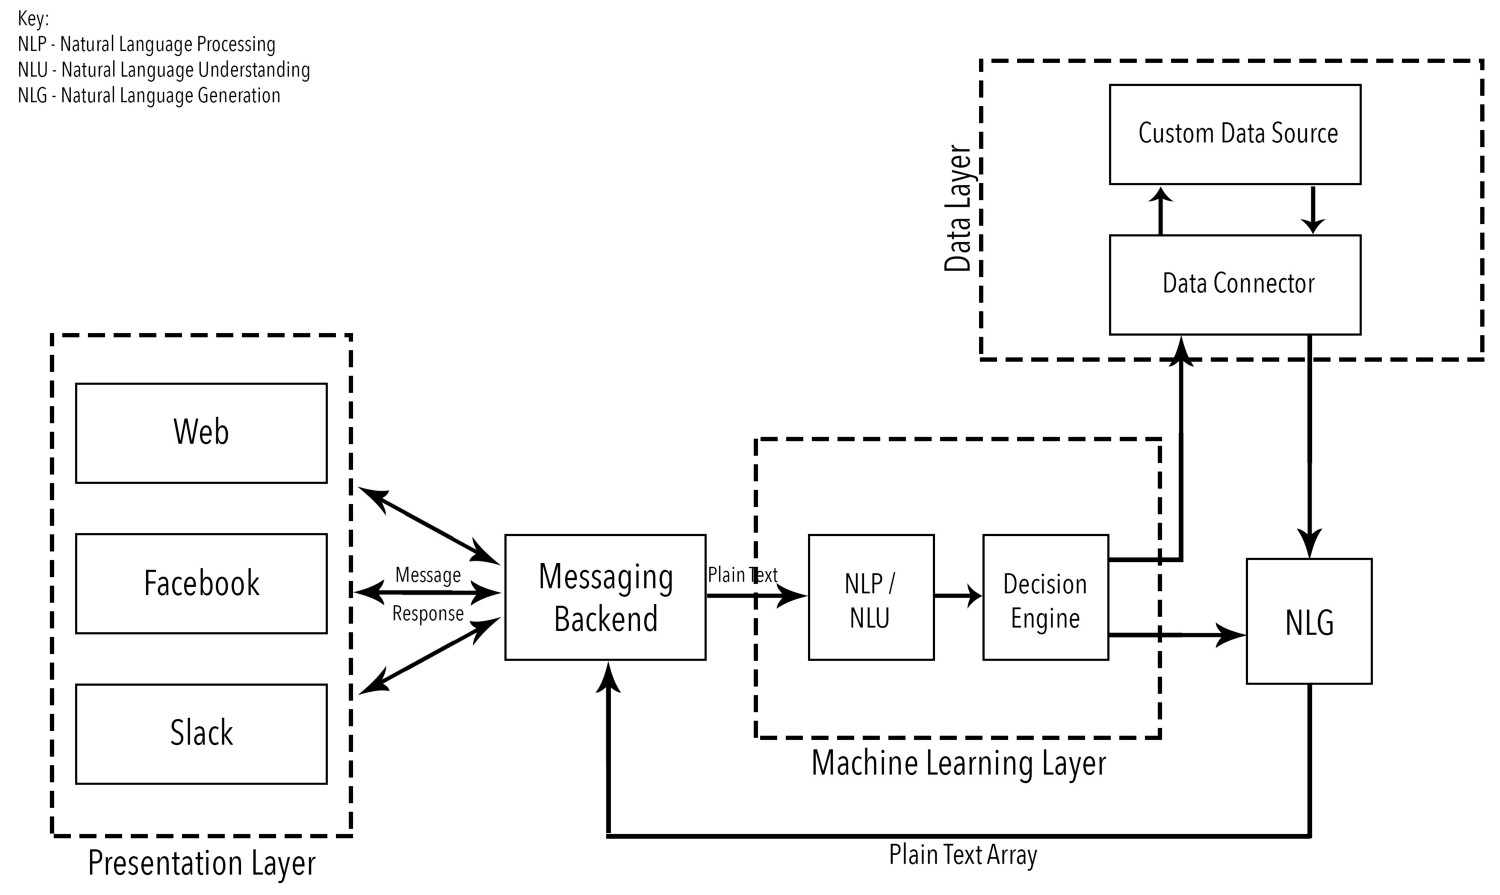
\includegraphics[scale=0.2]{nlschema}
		\caption{NLP, NLU, NLG and how Chatbots work.\cite{nlpnlunlg}}
	\end{figure}
	\begin{itemize}
	\item \textit{NLP} is the biggest set between the three, because it's a term which indicates the capability of a software to ingest an input sentence, split it in pieces (entities), understand the entities and their relationship, and give the answer to the user.
	
	\item \textit{NLU} is a subset of \textit{NLP}. It deals with understanding a natural language input (totally or partially unstructured) and convert it into a structured form that the machine can process and understand. Is a small yet critical task to achieve.
	
	\item \textit{NLG} can be seen as the dual phase of \textit{NLU}: turning structured data into natural language, to give the user the answer he wants.
	\end{itemize}
	
	\section{How can machine learning help NLU?}
	\subsection{Attention-Based RNN model for joint intent detection and slot-filling}
	One interesting work that can help in understanding the strong relationship between natural language understanding and machine learning, can be the one by Bing Liu and Ian Lane\cite{rnn}. Intent detection and slot-filling are indeed crucial parts of NLU: intent detection can be seen as a classification problem were, given a set of words (the sentence), the algorithm is capable to classify that sentence and give it a label which will correspond to one of the intents that the machine is able to recognize. Slot-filling can be just seen as a sequence labeling task. Regarding the intent detection phase, the classification problem can be faced by popular machine learning algorithms like \textit{Neural Networks (NNs)} or \textit{Support Vector Machines (SVMs)}; instead, for the slot-filling sequence labeling task, useful tools can be \textit{Markov models (MEMMs)} and \textit{Conditional Random Fields (CRFs)}.\\\\
	Is fundamental in this case, to understand the concept of alignment:
	\begin{itemize}
		\item Alignment is present when the output of the encoder is the same input given to the decoder. Is the case of slot-filling, where the entire set of entities is aligned (when processed with the encoder, can be directly given to the decoder).
		
		\item Alignment is not present when the output of the encoder can't be directly given in input to the decoder. An additional processing phase is needed before feeding the decoder with the informations it needs as input. is the case of the intent detection, where the decoder needs the information of all the words to detect the intent.
	\end{itemize}
	In both intent detection and slot-filling tasks, \textit{RNNs (Recurrent Neural Networks)} can be (and have been) applied:\\\\
	In the case of slot-filling, the input-output sequence is explicitly aligned, with a "slot" to fill for each single information extracted from the sentence. The models used in the years, in this case, have the aim to maximize the likelihood:
	\begin{equation}
	\arg \max_{\theta} \prod_{t=1}^{T} P(y\textsubscript{t}|y\textsubscript{1}\textsuperscript{t-1},x;\theta)
	\end{equation}
	Another structure exploiting RNNs can be instead the RNN Encoder-Decoder framework: in this case the input-output sequence is not aligned, and this structure is of course better for an intent detection task. In this case, the encoder and the decoder are separated entities: the encoder reads a sequence of inputs into a context vector \textit{c}, which is used from the decoder as source of informations for fulfilling its task. The probability of the output sequence of the decoder is:
	\begin{equation}
	P(y) = \prod_{t=1}^{T} P(y\textsubscript{t}|y\textsubscript{1}\textsuperscript{t-1},c)
	\end{equation}
	The work conducted by Liu and Lane aims to propose two different alternatives to be able to work well in joint intent detection and slot-filling tasks.
	\begin{figure}[H]
		\centering
		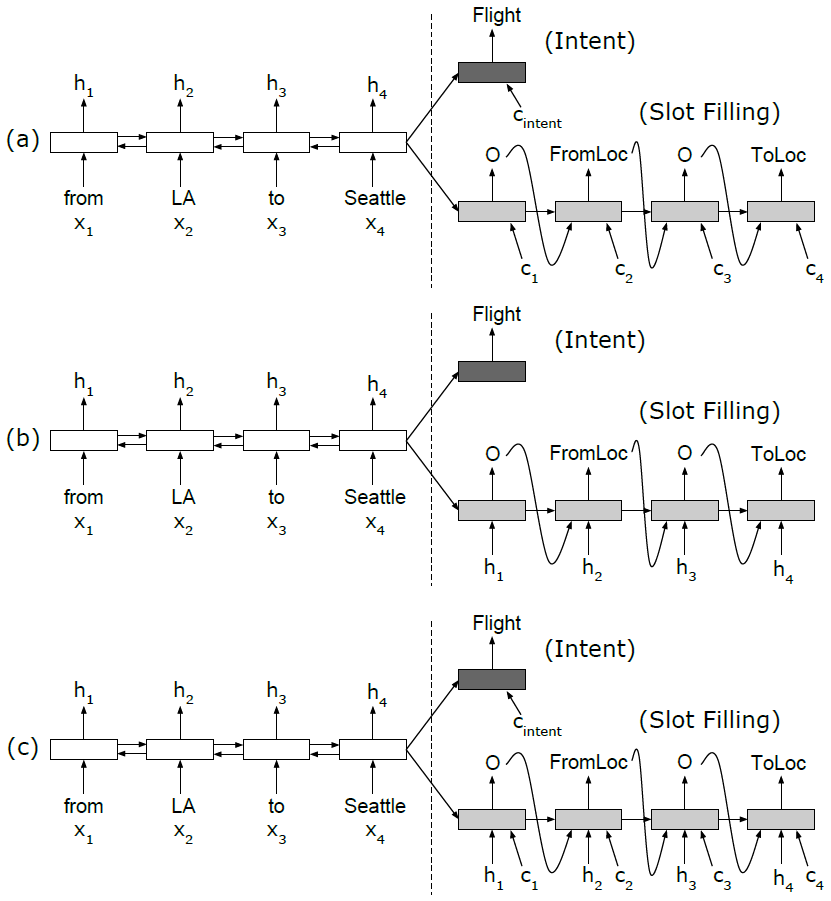
\includegraphics[scale=0.4]{alt1}
		\caption{The three alternatives using the Encoder/Decoder model.}
	\end{figure}
	In this case, as the figure shows, the encoder and the decoder phase are separated. In the encoder phase we can find the \textit{bidirectional RNNs}: each of them produces an hidden "forward" state \textit{fh\textsubscript{i}} and an hidden "backward" state \textit{bh\textsubscript{i}}. The output of the last \textit{RNN} is used for the intent detection and to initialize the decoder \textit{RNN} state.\\\\
	In the subfigure \textit{(a)}, we can find an example of non-aligned inputs. Indeed, the input given to the decoder phase is the context vector \textit{c}, produced by a weighted sum of all components of the \textit{h} vector produced by the encoder phase.\\
	In the subfigure \textit{(b)}, the inputs are aligned. The input vector of the decoder phase is just the \textit{h} array.\\
	The last subfigure \textit{(c)} shows a situation with aligned inputs and also the addition of attention. This is useful for the joint intent classification and slot-filling task: both the \textit{h} and the \textit{c} vectors are used in the decoder phase, that shows also an intent detection taking as input the output of the last \textit{RNN} and also the \textit{c} context vector.
	\begin{figure}[H]
		\centering
		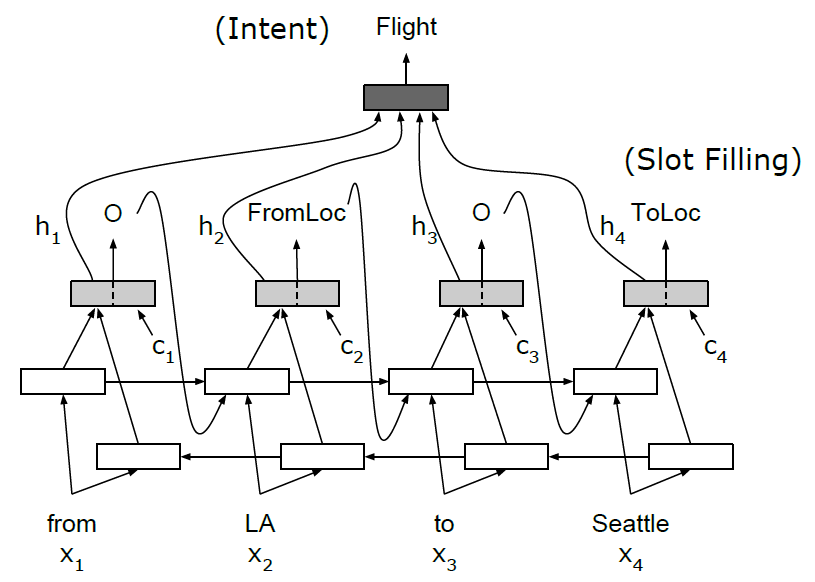
\includegraphics[scale=0.4]{alt2}
		\caption{Attention-based RNN model for joint intent detection
			and slot filling.}
	\end{figure}
	The attention-based model proposed by Liu and Lane shows a clear structure: each bidirectional \textit{RNN} produces a forward and a backward hidden state, useful for predicting the slot label (the core of the slot-filling task). At the same time, these outputs \textit{h\textsubscript{i}} are merged with the context vector \textit{c} to predict the final intent label.
	
	\subsection{A Unified Architecture for Natural Language Processing: Deep Neural Networks with Multitask Learning}
	One fundamental work in the Natural Language Processing worlds is the one by Collobert and Weston\cite{unified}. In their work, they propose a deep neural network that learns relevant features also with limited prior knowledge.\\\\
	The different tasks considered in the work are:
	\begin{itemize}
		\item Part-Of-Speech Tagging (POS): labeling each word with its role in the sentence (noun, adverb, verd, etc.).
		\item Chunking: labeling segments of sentences, with each word tagged as begin-chunk or inside-chunk.
		\item Named Entity Recognition (NER): labels elements in the sentence in categories (person, city, company, etc.).
		\item Semantic Role Labeling (SRL): gives a semantic role to a constituent of a sentence.
		\item Language Models: estimates the probability of the next word to be \textit{w} in a given word sequence.
		\item Semantically Related Word: understand if two words are semantically related (synonyms, holonymns, etc.).
	\end{itemize}
	\begin{figure}[H]
		\centering
		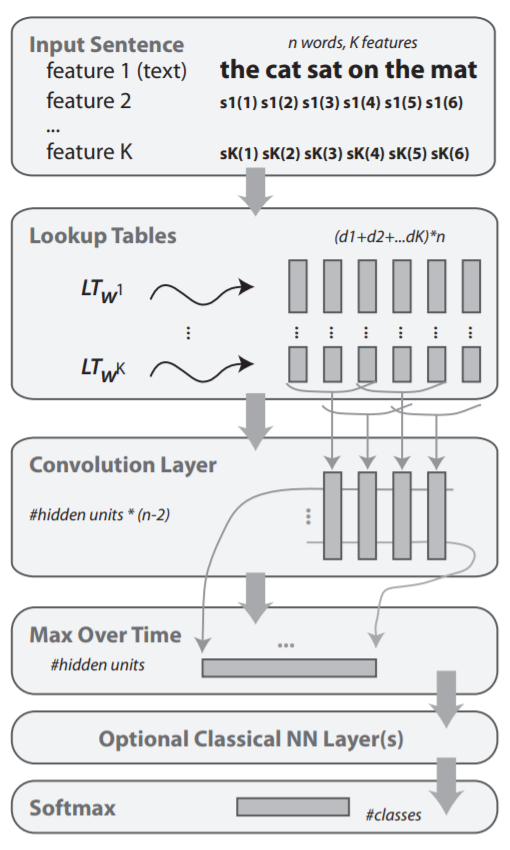
\includegraphics[scale=0.4]{unified}
		\caption{Deep Neural Networks for Natural Language Processing\cite{unified}.}
	\end{figure}
	In the proposed model, each word is considered as part of a given table:
	\begin{equation}
	LT_w(i) = W_i
	\end{equation}
	where the W term is the set of parameters to be learned. So, in the first layer of the network the input sequence is transformed into a set of vectors ${W_i}$.\\\\
	The output is then computed by the second layer, which performs convolutional operations:
	\begin{equation}
	o(t) = \sum_{j=1-t}^{n-t} L_j \cdot x_{t+j}
	\end{equation}
	where the \texttt{L} parameters are trained by back-propagation.\\\\
	Then, a layer follows the convolutional ones: it takes the most relevant features of the sentence feeding the output into a "\textit{Max}" Layer. It's important to notice that the output is of fixed length: this means that classical neural networks can be appended and trained for the labeling tasks.\\\\
	An important feature of the proposed model is the ability to perform multitask learning (MTL), in a deep joint training fashion. The network automatically learns features for each task in the various layers of the architecture: the deepest layers (with lookup-tables) learns the features for each word in the dictionary, so using them in common for related tasks (during training) can improve the overall generalization performance. In the work proposed by Collobert and Weston indeed, training is done in a stochastic fashion (keeping in mind that the labeled data for each task can be different, also coming from different datasets):
	\begin{enumerate}
		\item Take the next task.
		\item Select a training example for this specific task.
		\item Train the neural network (updating weights) using the gradient with respect to the example.
		\item Restart from point 1.
	\end{enumerate}

	\section{State of art: famous and most used tools}
	\begin{itemize}
		\item \textbf{Dialogflow}\cite{dialogflow}\\
		Google owned, is a rich solution in terms of machine learning.
		
		Pros:
		\begin{itemize}
			\item It's free and it has an easy documentation to start with.
			\item Entities or parameters can be marked as required (fundamental for the slot-filling process).
			\item Lots of languages supported.
		\end{itemize}
		
		Cons:
		\begin{itemize}
			\item No evaluation metrics.
			\item Not so smart with non-English languages.
			\item No spell-checking service offered.
		\end{itemize}
		
		\item \textbf{Wit.ai}\cite{witai}\\
		Facebook owned, is one of the most complete solutions for natural language processing. It supports 50 languages, it’s free.
		
		Pros:
		\begin{itemize}
			\item Supports machine learning to learn alternative phrases.
			\item UI to work with intent and entities.
			\item Developer view with conversation flows, context variables, branching logic.
			\item Supports "roles" in entities (e.g. \texttt{fromLocation(Nice)} to \texttt{toLocation(Turin)}).
		\end{itemize}
		
		Cons:
		\begin{itemize}
			\item No "required field" option (slot-filling).
		\end{itemize}	

		\item \textbf{Snips}\cite{snips}\\
		An open source alternative to the most popular NLU systems.
		
		Pros:
		\begin{itemize}
			\item Fully runs on device.
			\item Heavily exploits machine learning (especially CRF).
			\item Privacy by design.
			\item Precise performance metrics .
			\item Open source\cite{snips}.
			\item Integrated Automatic Speech Recognition.
		\end{itemize}
		
		Cons:
		\begin{itemize}
			\item Doesn't support a big set of languages.
			\item The training is not so straightforward.
			\item No excellent documentation.
		\end{itemize}
	
		\item \textbf{Others}:\\
		IBM Watson\cite{watson}, Amazon Lex\cite{lex}, Microsoft LUIS\cite{luis}, Recast.ai\cite{recast}.
	\end{itemize}